\chapter{Econom\'ia}
%
%
Debido a la caracter\'istica meramente investigativa de \'este trabajo, solo
se exponen en este cap\'itulo posibles modelos de negocios alrederor del
\emph{Software Libre}, y algunos nichos de mercado que se encuentran siendo
explotados en la actualidad.\\

\section{Modelos de negocios}
% Contar o cambial la cantidad de categorias, ahora dice 9 pero van a ser mas
La organizaci\'on FLOSSMetrics 
(Free / Libre and Open Source Software Metrics
\footnote{V\'ease - \url{http://www.flossmetrics.org/}})
, que forma parte de la Flossquality (Open source quality research
\footnote{V\'ease - \url{http://www.flossquality.eu/}})
, ambos financiados por la Comisi\'on Europea
\footnote{Vease -
\url{http://cordis.europa.eu/fetch?CALLER=PROJ_IST&ACTION=D&RCN=79449}}
, postula varias categorizaciones
\footnote{V\'ease -
\url{http://smeguide.conecta.it/index.php/6._FLOSS-based_business_models}} 
de modelos de negocios potenciales.


%%%%%%%%%%%%%%%%%%%%%%%%%%%%%%%%%%%%%%%%%%%%%%%%%%%%%%%%%%%%%%%%%%%%%%%%%%%%%%%
\subsection{Financiaci\'on externa de empresas}\footnote{En ingl\'e
\emph{Externally funded ventures}}
%
Esta categoria contempla los grupos o compa\~nias que desarrollan
\emph{Software Libre} siendo financiados por una organizaci\'on externa.
Normalmente es \'esta organizacion externa quien pone las gu\'ias y
requerimientos para el proyecto. \'Esta categoria es luego desglosada en tres
partes segun el origen de la financiaci\'on.

\subsubsection{Financiaci\'on P\'ublica}\footnote{En ingl\'es \emph{Public
funding}}
%
Se refiere a aquellos proyectos que son financiados por entidades p\'ublicas.
\'Estos suelen ser proyectos cint\'ificos o desarrollo de estandares cuyo fin
\'ultimo no necesariamente es generar ganancias econ\'omicas si no m\'as bien
algun beneficio social.

\subsubsection{Financiaci\'on ``Necesidad de mejora''}\footnote{En ingl\'es
\emph{``Needed improvement'' funding}}
%
\'Esta es la situaci\'on donde una compa\~nia le paga a un grupo u otro
compa\~nia para que mejore o adapte (y quiz\'a m\'as tarde de soporte) de un
proyecto libre existente.

\subsubsection{Fundaci\'on Indirecta}\footnote{En ingl\'es \emph{Indirect
funding}}
%
Muchas veces ciertas compa\~nias financias proyectos de \emph{Software Libre}
como estarategia de negocio, para obtener, de manera indirecta, algun r\'edito
econ\'omico. El ejemplo m\'as comun es cuando un fabricante de \emph{hardware}
financia a alguien m\'as (muchas veces son sus mismos empleados trabajando
para proyectos de \emph{Software Libre}) para que escriba los \emph{drivers}
para un sistema operat\'ivo libre (como lo puede ser GNU/Linux). 

\subsection{Uso Interno}\footnote{En ingl\'es \emph{Internal use}}
%
En este caso, las empresas, optan por realizar un desarrollo propio (en vez,
de quiza, optar por una soluci\'on propietaria ya existente) para solucionar
algun problema en particular. Luego liberan el co\'odigo para beneficiarse de
las contribuciones que puede brindar la comunidad de \emph{Software Libre}.

\subsection{Mejor conocimiento aqu\'i sin limitaciones}\footnote{En ingl\'es
\emph{Best knowledge here without constraints}}
%
En este modelo, una empresa presta servicios como \emph{consultor externo} para
otra compa\~nia sacando r\'edito mediante el alto nivel de conocimiento de su
personal.
Este tipo de modelos favorece la competencia del mercado, ya que aquella
empresa que necesita consultor\'ia, puede elegir siempre al mejor postor,
obligando a quien provee el servicio a manterner precios competitivos y
asegurar un excelente nivel t\'ecnico en sus empleados.

\subsection{Mejor conocimiento aqu\'i con limitaciones}\footnote{En
ingl\'es \emph{Best knowledge here with constraints}}
%
Para prevenir el ``robo'' de clientes, una empresa puede proveer servicios
libres, pero mantener privativo (o con una licencia m\'as restrictiva) a una
peque\~na parte clave c\'odigo.

\subsection{Doble Licencia}\footnote{En ingl\'es \emph{Dual licensing}}
%
Un modelo muy explotado en el negocio del \emph{Software Libre} es el de doble
licenciamiento. En este modelo la empresa que desarrolla \emph{Software
Libre} otorga licencias libres para los proyectos que vayan a continuar siendo
libres (usualmente entregando el producto gratis) y una licencia distinta
(usualmente paga) para aquellas otras empresas que no deseen redistribuir el
c\'odigo. 

\subsection{Desarrollo no financiaciado}\footnote{En ingl\'es \emph{Unfunded
developments}}
%
Existen situaciones donde, si se da con suficiente \'enfasis un efecto de
\emph{networking}\footnote{En castellano \emph{red}. Es cuando por motivos
t\'ecnicos o sociales el proyecto obtiene una impacto importante en la
algunas comunidades de internet.}, requiere solo un esfuerzo minimo de la
organizaci\'on el publicar su producto, ya que la mayoria del aporte lo
obtiene de otras compa\~nias que por diversos intereses asignan recursos
dedicados a ese producto sin pretender un beneficio econ\'ominco inmediato.
Los casos m\'as comunes son las distribuciones de GNU/Linux (como
Debian\footnote{\url{http://www.debian.org/}}) o los sitemas operativos
basados en \emph{BSD}\footnote{\url{http://es.wikipedia.org/wiki/BSD}} (como
FreeBSD\footnote{\url{http://www.freebsd.org/}}). Pero el ejemplo m\'as
ilustre de todos es el proyecto
\emph{linux}\footnote{\url{http://www.kernel.org/}}, el cual es desarrollado
por un grupo muy reducido de personas, pero que recibe el aporte de miles de
% 'de alrededor del mundo' o sin el 'de' ????
desarrolladores de alrededor del mundo, muchos de los cuales pertenecen a
diversas empresas y son contratados para \'este trabajo dedicado.
La \emph{Linux Foundation}
public\'o\footnote{\url{
http://www.linuxfoundation.org/publications/whowriteslinux.pdf}} un
art\'iculo\footnote{Que se encuentra algo desactualizado debido a la rapida
evoluci\'on de este tipo de proyectos.} donde muestra el aporte de algunas de
las empresas m\'as importantes del mundo al proyecto linux como se puede
observar en la figura \ref{fig:companies_contributions_to_linux}.

% http://www.linuxfoundation.org/publications/images/table4-companies.gif
\begin{figure}[htp]
\centering
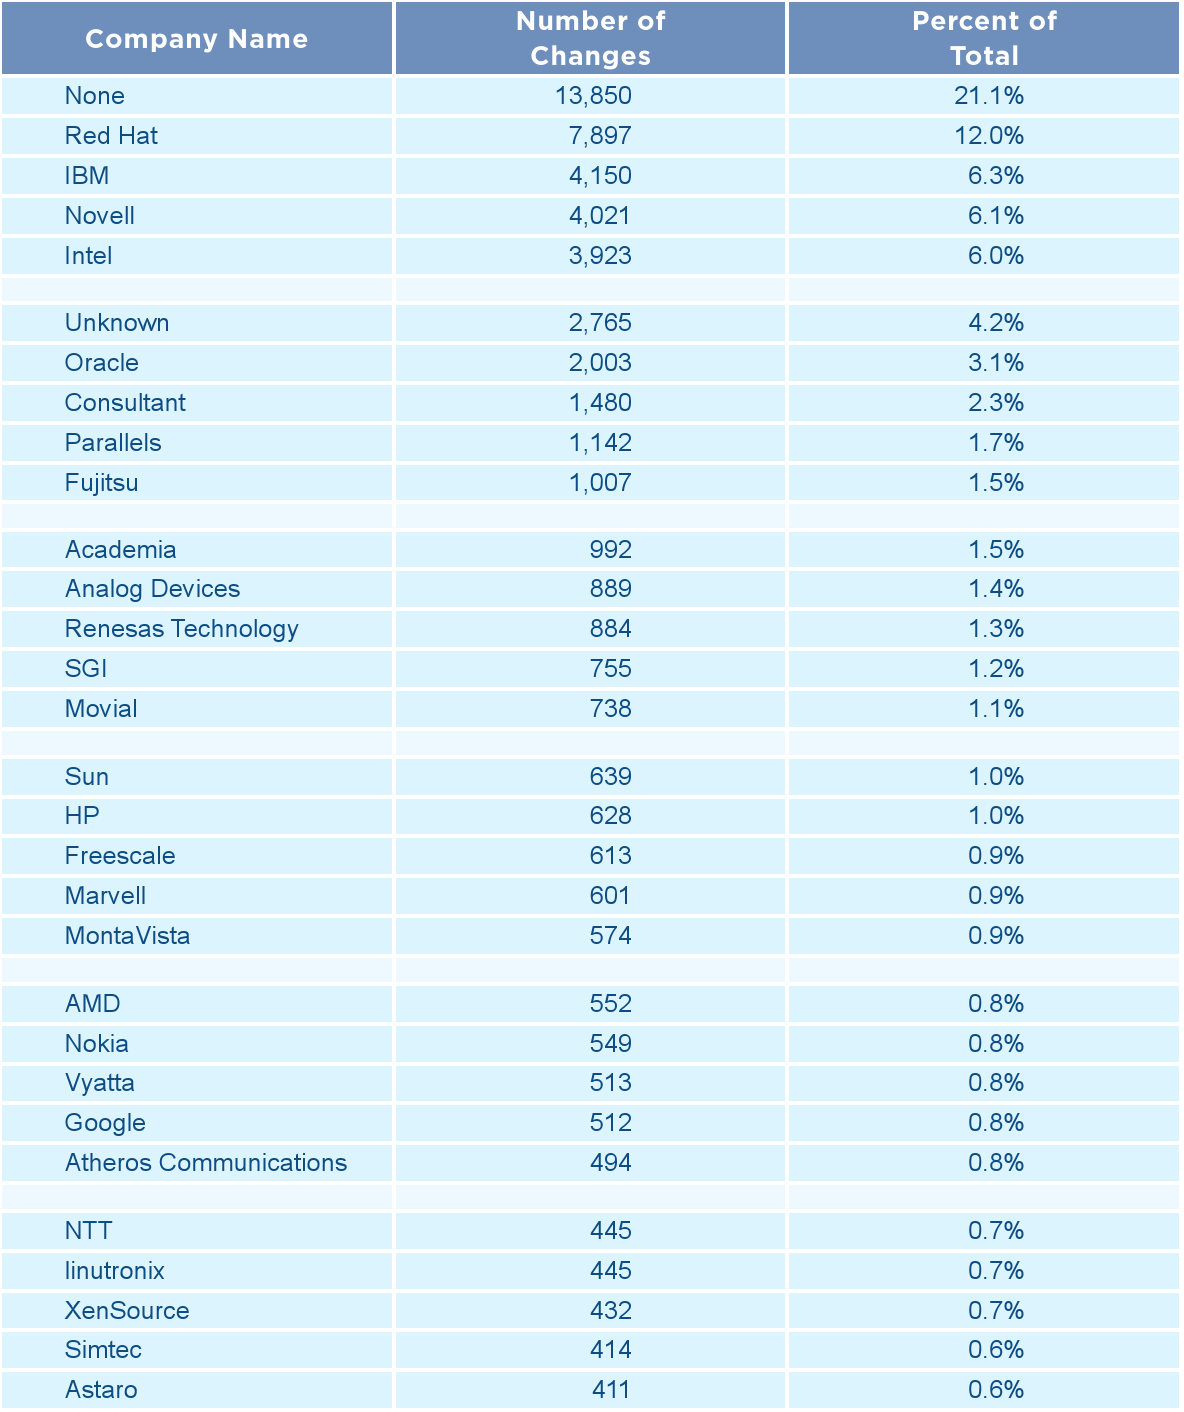
\includegraphics[width=13cm]{./img/table4-companies.png}
\caption{Contribuci\'on de diversas empresas al kernel de linux.}
\label{fig:companies_contributions_to_linux}
\end{figure}\footnote{Datos m\'as actualizados pueden ser generados
autom\'aticamente usando los \emph{scripts} disponibles en
\url{http://www.kernel.org/pub/linux/kernel/people/gregkh/kernel_history/}.}


\section{Posibles modelos particulares}
%
No es el fin de \'este proyecto obtener r\'edito econ\'omico alguno, sin
embargo puede ser de interes de alguien sacar provecho del trabajo aqu\'i
presentado, para ello se analiza a continuaci\'on algunos aspectos
econ\'omicos del mismo.

\subsection{Costos}
Los valores aqu\'i presentados son aproximaciones muy %burdas

Los precios usados son obtenidos de (en caso de ser posible) sus respectivos
fabricantes, o de grandes distribuidores en su defecto, asumiendo compras
mayores de 100 unidades, suponiendo as\'i que es una empresa en vista de
producci\'on en serie quien usar\'a los datos aqui presentados.

% PIC18F4550 = 4.26 USD
% http://www.microchipdirect.com/productsearch.aspx?Keywords=18f4550

% Conector USB B hembra = 0,37 €
% http://es.farnell.com/lumberg/2411-02/hembra-usb-panel-pcb-tipo-b/dp/1177885

% TIP 122 = 0,33 € 
%http://es.farnell.com/multicomp/tip122/transistor-darlington-to-220/dp/9294236
